% Options for packages loaded elsewhere
\PassOptionsToPackage{unicode}{hyperref}
\PassOptionsToPackage{hyphens}{url}
%
\documentclass[
  ignorenonframetext,
]{beamer}
\usepackage{pgfpages}
\setbeamertemplate{caption}[numbered]
\setbeamertemplate{caption label separator}{: }
\setbeamercolor{caption name}{fg=normal text.fg}
\beamertemplatenavigationsymbolsempty
% Prevent slide breaks in the middle of a paragraph
\widowpenalties 1 10000
\raggedbottom
\setbeamertemplate{part page}{
  \centering
  \begin{beamercolorbox}[sep=16pt,center]{part title}
    \usebeamerfont{part title}\insertpart\par
  \end{beamercolorbox}
}
\setbeamertemplate{section page}{
  \centering
  \begin{beamercolorbox}[sep=12pt,center]{part title}
    \usebeamerfont{section title}\insertsection\par
  \end{beamercolorbox}
}
\setbeamertemplate{subsection page}{
  \centering
  \begin{beamercolorbox}[sep=8pt,center]{part title}
    \usebeamerfont{subsection title}\insertsubsection\par
  \end{beamercolorbox}
}
\AtBeginPart{
  \frame{\partpage}
}
\AtBeginSection{
  \ifbibliography
  \else
    \frame{\sectionpage}
  \fi
}
\AtBeginSubsection{
  \frame{\subsectionpage}
}
\usepackage{lmodern}
\usepackage{amsmath}
\usepackage{ifxetex,ifluatex}
\ifnum 0\ifxetex 1\fi\ifluatex 1\fi=0 % if pdftex
  \usepackage[T1]{fontenc}
  \usepackage[utf8]{inputenc}
  \usepackage{textcomp} % provide euro and other symbols
  \usepackage{amssymb}
\else % if luatex or xetex
  \usepackage{unicode-math}
  \defaultfontfeatures{Scale=MatchLowercase}
  \defaultfontfeatures[\rmfamily]{Ligatures=TeX,Scale=1}
\fi
% Use upquote if available, for straight quotes in verbatim environments
\IfFileExists{upquote.sty}{\usepackage{upquote}}{}
\IfFileExists{microtype.sty}{% use microtype if available
  \usepackage[]{microtype}
  \UseMicrotypeSet[protrusion]{basicmath} % disable protrusion for tt fonts
}{}
\makeatletter
\@ifundefined{KOMAClassName}{% if non-KOMA class
  \IfFileExists{parskip.sty}{%
    \usepackage{parskip}
  }{% else
    \setlength{\parindent}{0pt}
    \setlength{\parskip}{6pt plus 2pt minus 1pt}}
}{% if KOMA class
  \KOMAoptions{parskip=half}}
\makeatother
\usepackage{xcolor}
\IfFileExists{xurl.sty}{\usepackage{xurl}}{} % add URL line breaks if available
\IfFileExists{bookmark.sty}{\usepackage{bookmark}}{\usepackage{hyperref}}
\hypersetup{
  pdftitle={Impact of Government Expenditure in Education on Unemployment},
  pdfauthor={Anna Canestro, Serena Foini \& Catherine Vanaise},
  hidelinks,
  pdfcreator={LaTeX via pandoc}}
\urlstyle{same} % disable monospaced font for URLs
\newif\ifbibliography
\usepackage{graphicx}
\makeatletter
\def\maxwidth{\ifdim\Gin@nat@width>\linewidth\linewidth\else\Gin@nat@width\fi}
\def\maxheight{\ifdim\Gin@nat@height>\textheight\textheight\else\Gin@nat@height\fi}
\makeatother
% Scale images if necessary, so that they will not overflow the page
% margins by default, and it is still possible to overwrite the defaults
% using explicit options in \includegraphics[width, height, ...]{}
\setkeys{Gin}{width=\maxwidth,height=\maxheight,keepaspectratio}
% Set default figure placement to htbp
\makeatletter
\def\fps@figure{htbp}
\makeatother
\setlength{\emergencystretch}{3em} % prevent overfull lines
\providecommand{\tightlist}{%
  \setlength{\itemsep}{0pt}\setlength{\parskip}{0pt}}
\setcounter{secnumdepth}{-\maxdimen} % remove section numbering
\ifluatex
  \usepackage{selnolig}  % disable illegal ligatures
\fi

\title{Impact of Government Expenditure in Education on Unemployment}
\author{Anna Canestro, Serena Foini \& Catherine Vanaise}
\date{05/04/2021}

\begin{document}
\frame{\titlepage}

\begin{frame}{Agenda}
\protect\hypertarget{agenda}{}
\begin{enumerate}
\tightlist
\item
  Background
\item
  Research Gap
\item
  Hypotheses Formulation
\item
  Methodology
\item
  Data Analysis\\
\item
  Discussion
\item
  Conclusion
\end{enumerate}
\end{frame}

\begin{frame}{Background}
\protect\hypertarget{background}{}
Unemployment levels are constantly under the spotlight of governments,
as signals of the economic stability of countries and of the
effectiveness of the policies they implement. It is conventionally
believed that the acquisition of skills enhances the possibilities of
getting hired (Grimaccia \& Lima, 2013). Previous investigated three
important relationships:

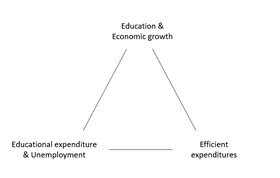
\includegraphics{./Immagine2.png}
\end{frame}

\begin{frame}{Research Gap}
\protect\hypertarget{research-gap}{}
Despite the large amount of research on the relationship between
educational expenditure and both economic growth and unemployment,
\textbf{a large gap in the literature is found regarding the division of
these expenditures among the different educational levels.}

\begin{enumerate}
\tightlist
\item
  It is not investigated whether and how investments in a particular
  level of education -- primary, secondary or tertiary -- provide
  greater benefit on the economy.
\item
  The literature generally focuses more on specific-countries rather
  than cross-country studies, which could be extremely helpful in the
  view of resources allocation decisions.
\end{enumerate}
\end{frame}

\begin{frame}{Our Aim}
\protect\hypertarget{our-aim}{}
The aim of our research is to assess whether the expenditure in
education is negatively correlated to unemployment levels. We studied
whether the impact of government expenditures in education on
unemployment varies according to the destination of these expenditures
-- primary, lower and upper secondary, tertiary schooling. This research
aims at, better understanding on which educational level governments
should direct their investments to reach the best possible outcome for
diminishing unemployment.
\end{frame}

\begin{frame}{Hypothesis Formulation}
\protect\hypertarget{hypothesis-formulation}{}
\textbf{Hypothesis 1:} Higher government investments in primary
education will lead to lower unemployment rates

\textbf{Hypothesis 2:} Higher government investments in lower secondary
education will lead to lower unemployment rates.

\textbf{Hypothesis 3:} Higher government investments in upper secondary
education will lead to lower unemployment rates.

\textbf{Hypothesis 4:} Higher government investments in long-cycle
tertiary education will lead to lower unemployment rates.
\end{frame}

\begin{frame}{Methodology}
\protect\hypertarget{methodology}{}
We used panel data gathered from the OECD.Stat, which reports data from
the 38 OECD members. We included only 26 countries in our sample as 12
of the countries were missing too much information to be properly
analyzed. This samples allows for a cross country analysis.

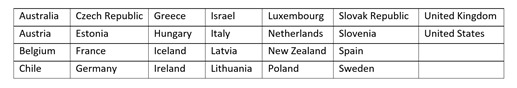
\includegraphics{./Table of countries.jpeg}

Despite the sample of OECD countries being downsized, we were careful to
maintain geographical heterogeneity.\\
We decided to limit the scope of our analysis to the period from 2013 to
2017 since they were the five most recent years available.
\end{frame}

\begin{frame}{Variables}
\protect\hypertarget{variables}{}
\begin{block}{Dependent Variable}
\protect\hypertarget{dependent-variable}{}
Our dependent variable is the level of unemployment. It is measured as
the percentage of the population aged between 24 and 64 years of age
that is without employment.
\end{block}

\begin{block}{Independent Variable}
\protect\hypertarget{independent-variable}{}
\begin{enumerate}
\tightlist
\item
  The level of total expenditure in primary education (ISCED2011 level
  1);
\item
  The level of total expenditure in lower secondary education (ISCED2011
  level 2);
\item
  The level of total expenditure in upper secondary education (ISCED2011
  level 3);
\item
  the level of total expenditure in long cycle tertiary education
  (ISCED2011 levels 6 to 8).
\end{enumerate}

They are all included in the model as percentage of the GDP of the
specific country in order to normalize with respect to the economic
development of the different nations.
\end{block}
\end{frame}

\begin{frame}{Control Variables}
\protect\hypertarget{control-variables}{}
\begin{enumerate}
\tightlist
\item
  The educational attainment measures the percentage of university
  graduates in the population aged 25-64 and controls for the social
  recognition of education.The higher the percentage of people with
  tertiary education, the greater the recognition of this attainment in
  the social and labor environment.
\item
  The student-teacher ratio is used as a proxy of the quality of the
  schooling system in a specific country: it is assumed that the lower
  the number of students per teacher, the greater the attention
  dedicated to each of them.
\end{enumerate}
\end{frame}

\begin{frame}{Categorical Variables}
\protect\hypertarget{categorical-variables}{}
\begin{block}{Geographical categorization}
\protect\hypertarget{geographical-categorization}{}
We classified countries by their geographical region---South America,
North America, Western Europe, Eastern Europe, Northern Europe, Middle
East and Oceania. We did not distinguish Southern Europe as the three
countries that formally belong to this group---Italy, Spain and
Greece---could be grouped in the previously defined categories. In this
case, the base category is Middle East.
\end{block}

\begin{block}{Income categorization}
\protect\hypertarget{income-categorization}{}
We classified countries by their level of income, according to the GDP
per capita. Since, by the classification of The World Bank (2021), they
all belong to the high-income cluster, we proceeded with a further
division by quartiles and to each of them we associated low-, lower
middle-, upper middle-, and upper-income categories. In this case, the
base category is represented by low-income countries.
\end{block}
\end{frame}

\begin{frame}{Data Analysis}
\protect\hypertarget{data-analysis}{}
\begin{block}{Explanatory data analysis}
\protect\hypertarget{explanatory-data-analysis}{}
Our 130 observations are arranged in form of panel data and we used
time-series cross-section-based estimation techniques. PUT THE TABLE OF
SUMMARY STATISTICS
\end{block}
\end{frame}

\begin{frame}{Modeling}
\protect\hypertarget{modeling}{}
PUT THE MODELS
\end{frame}

\begin{frame}{Validity}
\protect\hypertarget{validity}{}
From the previous results, we concluded that the unique model which
provides us with significant outcomes is model (3). It is important to
test its validity, hence whether we collected the right data. To do so
we looked at three conditions: linearity, distribution and variability
of residuals.
\end{frame}

\begin{frame}{Linearity}
\protect\hypertarget{linearity}{}
Concerning the linearity conditions, plotting model (3) in a Cartesian
plane, except for some outliers, the relationship resembled a linear
one. To be more confident, we decided to test the quadratic effect.
However, the quadratic term was dropped, implying that its effect is
null. Hence the model should be linear, increasing its validity.
\end{frame}

\begin{frame}{Distribution of residuals}
\protect\hypertarget{distribution-of-residuals}{}
To test the distribution of the residuals, they have been plotted in a
histogram which represented symmetric residuals around zero. The
skewness test gave a g\_1 for our residuals smaller than the theoretical
threshold 2*sqrt(6⁄n). This confirmed our first impression from the
graph, that there is no skewness, strengthening model's validity.

PLOT OF THE RESIDUALS
\end{frame}

\begin{frame}{Residuals Homoskedasticity}
\protect\hypertarget{residuals-homoskedasticity}{}
The last condition to be verified was the residuals' homoskedasticity.
We applied the Breusch-Pagan test which gave us a p-value of 2.2e-16
which is much lower the 5\% significance level, implying
heteroskedasticity. Heteroskedasticity might deeply affect the validity
of our findings, however a way to obtain robust coefficients is through
the t-test on the latter. Since we obtained a significant beta for our
dependent variable in model (3), we were able to mitigate this
limitation. To conclude, the overall validity of the model was moderate:
the tests showed some confidence of linearity, no skewness but the
presence of heteroskedasticity.
\end{frame}

\begin{frame}{Discussion}
\protect\hypertarget{discussion}{}
\textbf{None of our initial hypotheses can be accepted.} Data only
highlight a significant and---opposite from what expected---positive
relationship between long-cycle tertiary education expenditures and
unemployment rates.

\begin{block}{What does it mean?}
\protect\hypertarget{what-does-it-mean}{}
Despite the imperative to provide and spend in lower grades of
schooling, the effects of these investments are not directly captured by
unemployment levels. Following, the positive relationship between
unemployment rates and outlays in long-cycle tertiary education might
appear counter-intuitive. However, it tells us that countries which
spend more in higher education for more educated individuals who put
upward pressure to labour supply. If the latter is not matched by a
sufficient labour demand, it leads to an increase in unemployment rates,
which is the exact mechanism experienced in the countries of our sample.
\end{block}
\end{frame}

\begin{frame}{Conclusions}
\protect\hypertarget{conclusions}{}
\begin{block}{Limitations}
\protect\hypertarget{limitations}{}
Data were not available for all the OECD countries and, therefore, we
were forced to restrict our analysis to just 26 of them and for the
period between 2013-2017. This led us to further limitations when
considering possible division among countries, all of them being
categorized as high-income by the World Bank. Moreover, our study being
one of the firsts to focus on governmental expenditures broken down by
different schooling levels, we decided not to distinguish unemployment
among different ages but to consider general levels for the workers aged
25-64. Nonetheless, it is too broad of a group, and it is likely
subjected to other factors apart from government spending in education.
\end{block}
\end{frame}

\begin{frame}{Further Research}
\protect\hypertarget{further-research}{}
We suggest broadening the time frame, and considering a greater sample
of countries---from various regions and with different levels of
income---to increase the generalizability of the study. Secondly, future
analysis should consider as a dependent variable a smaller percentage of
the working population, preferably focusing on younger individuals to
better assess the real impact of expenditures on their hiring
possibilities. Lastly, different types of relationships could be
investigated -- i.e., the logarithmic form.

On the basis of these considerations, we thoroughly described all the
steps made to make our study reproducible and so to be used as a
reference for future studies in the field.
\end{frame}

\end{document}
